\subsection{Frequently asked Questions}

The list below is the question and answers to date.  We'll add more
question and answers as they come up, and fill out the answers below
as we get more information from other parties.

Q: Details on search function (on presentation pages as well as in
Content server)

A: Any content you put in your website will be full text indexed and
searchable globally.  However, if you modify the security for any
content, that security specification will be honored in the
search...that is people without permission will NOT see content they
don't have security permissions to see.  In addition to full-text
indexing (and searching) some metadata fields will also be indexed,
and some will not be.  We need to get a list of which ones are indexed
and which ones are not.

It seems that there was some difficulty with Japanese characters in a
metadata field, and having those show up.  We will raise an SR to
trouble shoot this issue.


Q: How to specify a relative path in the HTML editor.

A: Although there are mechanisms to use relative paths, it is
considered best practice to add links within content using
Contributor's link interface (within contributor data files, use the
link icon to launch) and reference links within Word using the full
path but replace the server name using \emph{httpserverrelativewebroot}
token.

When you use the Contributor linking mechanism, as broken link checks
can also be performed BEFORE they are deployed, using the link manager
extension.  For example when you link to a piece of content, then try
to delete that content, you will be warned that there are links
pointing to that link...so broken links are prevented before they
occur.

Q: How to use style sheet.

A: Stylesheets can be used in principle, but with the site that is
deployed we are currently restricted in what we can contribute to the
website.  We cannot include HTML or IDOC script at this point, so in
some sense the discussion around stylesheets is to little avail.


Q: Any tip when using external HTML editor like Dreamweaver.

A: We recommend against using external editors like Dreamweaver.
Dreamweaver creates HTML from WYSIWYG editor.  This is the same
functionality that Site Studio Contributor does and you cannot modify
this aspect of the standard Site Studio workflow without rendering the
whole system defunct.  It is the assumption that you can create pretty
much any layout you need with Site Studio Contributor.  If there are
features/techniques you cannot reproduce, the we can look at those
individually.

Q: How to specify images on a navigation tab.

A: Again, this won't be possible with the level of control the site
designers have delegated to the departments. If absolutely essential
we can look at ways to achieve this for you, but if the requirement
isn't exceptionally strong then it will be hard to justify the effort
required to achieve this.

Q: How to highlight a selected tab on a navigation when the page is
selected.

A: This is controlled by the CSS using hover, active and other common
link styles.  However, since we are not given access to the underlying
HTML/CSS we cannot make this change with the permissions to the system
we have.

Q: How to specify a URL for it when we locate a HTML file in a content
server, (....html? or CNT...?)

A: Use the built in link icon in Contributor.  To reference links
within Word use the full path but replace the server name using
\emph{httpserverrelativewebroot} token.

Q: What is the difference among Dynlistbox, Editorbox, and Editor. How
to use Query Text in Editor.

A: Here is a picture of an `EditorBox' as viewed by a visitor to the website:

\begin{figure}[h!]
  \centering
  \fbox{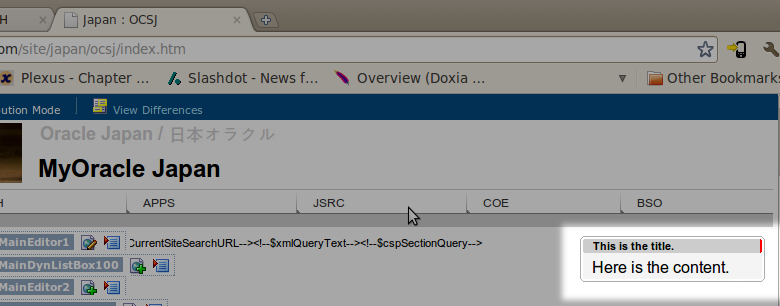
\includegraphics[width=130mm]{images/editorBox}}
  \caption{What an `Editor Box' looks like.}
\end{figure}

\clearpage

Here is a picture of the Contributor application when editing an
`Editor' region:

\begin{figure}[h!]
  \centering
  \fbox{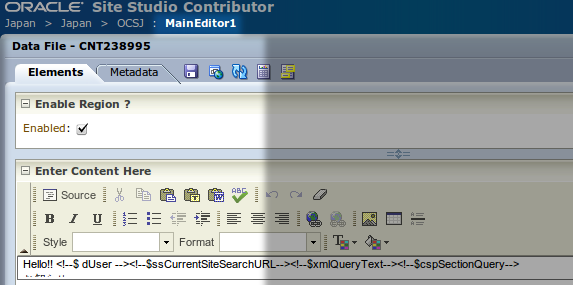
\includegraphics[width=130mm]{images/editor}}
  \caption{What an `Editor Box' looks like.}
\end{figure}

\clearpage

Finally, here is an image of the Contributor application when editing
an `EditorBox' element.  You'll notice an extra title field.

\begin{figure}[h!]
  \centering
  \fbox{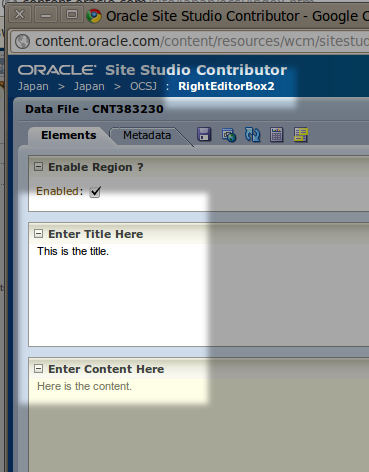
\includegraphics[width=130mm]{images/EditorBoxContributor}}
  \caption{What an `Editor Box' looks like.}
\end{figure}

\clearpage

Q: Should all the images be specified as CNTxxx files? if so, is there
any effective way of editing pages because it's a little bothering to
check its content ID every time when we upload an image file and
change the image URL to CNTxxx on a HTML.

A: Yes all images should be checked into the content server.  However,
I recommend the use of Desktop Integration Suite (DIS).  DIS is an
extension to windows explorer that lets you drag and drop files into
the content server.  Then you can display the title (which comes from
the filename) and the content id side by side so as to ease the
migration pain...no separate upload is required then.

Q: Workflow function.

A: I will have to do a review of the workflow that has been specified
for your team.  That requires that I coordinate with the implementors
of the site.  I will CC you on all communications.

Q: How to create a private page template if possible.

A: Security is controlled by metadata.  If you specify the correct
metadata then the page should only be visible to those that have
permission to access it.  However, we need to find out what the
security model of Oracle is to see if there are accounts that are put
aside to allow for private data.

Q: How to use Keywords in a content.

A: You can put keywords in a metadata field that is indexed.  I
believe we can use the xComments metadata field for this, as that
field should be indexed.  Of course any word that exists in your page
will become a keyword too, as the full page is full text indexed.  It
has been identified that there seems to be some issues with this and
Japanese characters, so we'll have to deal with this by raising a
Service Request.


Q: How to use the following properties on a presentation page: 
\begin{itemize}
\item cspSectionQuery
\item xmlQueryText
\item ssCurrentSiteSearchURL
\end{itemize}

A: The ability to add IDOC script to contribution sections is
controlled by the designers of the website.  It appears that they have
turned off the ability to include IDOC script on the websites they
have launched to the different departments...so as a result we won't
be able to specify or leverage any IDOC script.